\section{Introduction}\label{sec:intro}

\begin{figure*}[tp]
\centering
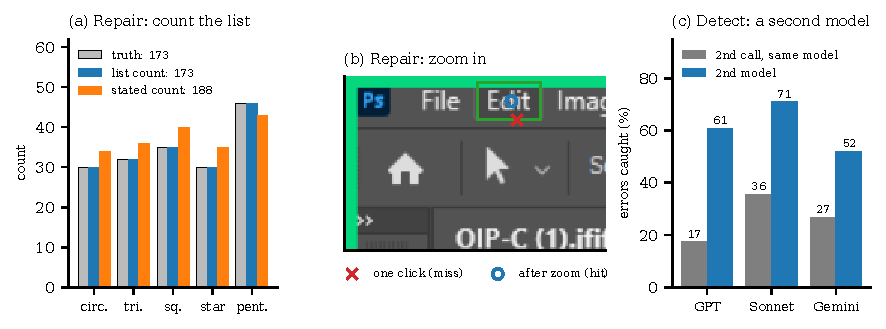
\includegraphics[width=\textwidth]{figures/fig_teaser.pdf}
\caption{Three lessons in one figure. (a) One response of GPT-6.1 to a dense synthetic scene (SCP-dense image 28, Section~\ref{sec:experiments}; 173 shapes of five classes). Grey: true number of shapes per class. Blue: the \emph{list count}, the number of records of each class in the model's list, counted by code; every one of its 173 records matches a different shape. Orange: the \emph{stated count}, the numbers the model wrote for each class in the same response; they sum to 188. Across 50 such scenes, the full list-first reporting and decoding protocol cuts per-type count error by 85.2\% (Section~\ref{sec:res:readout}). (b) A single click by Gemini 3.8 misses the ``edit menu'' (green box); a second call on a zoomed crop (ReGround, \citealp{li2025screenspotpro}) hits it. Two-stage zoom cuts its click error by 65\% (Section~\ref{sec:res:view}). (c) Miss rate against cost per item on 600 ScreenSpot-Pro items: GPT-6.1's two-stage zoom, three such zooms with a cluster vote, a crop-first baseline in the style of GUI-Lens \citep{fu2026guilens}, a plain vote over three models' zoomed points, and the three-model tier of Algorithm~\ref{alg:clicks}, which selects among the same points and keeps every item in the denominator (Section~\ref{sec:res:choose}).}
\label{fig:teaser}
\end{figure*}

Vision-language models are now asked to report a set of objects in an image: to count them, to box them, to parse every element of a screen, or to pick the one element a user means. A typical answer has two parts. The first is a \emph{list}: one entry per object, each giving a class name and a location (a point or a box). We call each entry a \emph{record}. The second, when it is requested, is a \emph{stated count}: the numbers the model writes for how many objects of each class it found. Code can also count the records in the list; we call that the \emph{list count}. The two counts should agree. Often they do not.

Figure~\ref{fig:teaser}a shows one response of GPT-6.1 to a dense synthetic scene with 173 shapes of five classes. Its list has 173 records, and each record matches a different shape of the same class within 20 pixels, so the list is exact. In the same response, the model states counts that add up to 188. Across 50 such scenes, GPT-6.1 wrote an exact list in 20 scenes, and in 19 of them its stated counts were wrong. Sonnet 5.5 wrote an exact list in 39 scenes (after mapping its word ``diamond'' to the class ``square''), and its stated counts were wrong in all 39. The response contains a correct enumeration; the model's own summary of that enumeration is not faithful to it.

Visual set reports are becoming the interface between perception models and the systems that use them: inventory counts, document layout, screen parsing for computer-use agents, click targets. Practitioners compensate with folklore: ask again, ask the model to check itself, overlay a grid, tell it not to miss anything, vote across models. Some of these help, some do nothing, and some make things worse. Without a model of where reporting errors come from, it is hard to predict which. Our thesis is that \emph{reporting is part of the visual task, not merely its formatting}: what a model delivers depends on how it is asked to report, how the report is decoded and read, and how several reports are combined, and each of these steps can be analysed and improved.

\paragraph{What we do.} We describe reporting as a chain with four objects (Figure~\ref{fig:chain}): a \emph{response}, the raw text of one call to a model; the \emph{records} decoded from it; a \emph{set} of records built from one or more responses, for example by keeping only records that two calls agree on; and the \emph{task answer} read from that set, such as a count per class or a click point. Three quantities connect the chain to every loss we study: the maximum number of records that can be paired one-to-one with true objects under the task's matching rule, the number of records that are scored, and the rule that reads the answer. They give exact relations for what each operation does. Deleting unconfirmed records lowers the error exactly when the deletion loses fewer than one match per two scored records removed (with equal costs of the two error types), whichever model or view supplied the confirmation. Averaging the coordinates of agreeing records is a separate effect that can help or hurt. The chain takes reports as they come: from one call on the whole image, or from several views produced by an existing view planner such as tiling or zoom, whose merging and cross-view confirmation are constructions like any other. Alongside these relations we state a behavioural model, kept separate from them: each object has a persistent tendency to be reported or missed, partly shared across models. This analysis of what a model reports complements analyses of what a single call can see \citep{shi2026zoomin}.

\begin{figure*}[tp]
\centering
\resizebox{\textwidth}{!}{%
\begin{tikzpicture}[
  box/.style={draw, rounded corners=2pt, align=center, font=\small, minimum height=1.05cm, inner sep=3pt, fill=white},
  arr/.style={-{Latex[length=2mm]}, thick},
  lab/.style={font=\footnotesize, align=center, text=black!70},
  stp/.style={draw, rounded corners=2pt, align=left, font=\footnotesize, inner sep=3pt, text width=3.3cm, minimum height=2.35cm, anchor=north},
  rep/.style={stp, fill=green!7, draw=green!45!black},
  wide/.style={draw, rounded corners=2pt, align=left, font=\footnotesize, inner sep=3pt, text width=7.2cm, minimum height=1.45cm, anchor=north},
  det/.style={wide, fill=orange!9, draw=orange!70!black},
  jud/.style={wide, fill=blue!6, draw=blue!60!black},
  link/.style={-{Latex[length=1.5mm]}, densely dashed, black!55}]
\node[box] (x) at (0,0) {image $x$\\task $\tau$};
\node[box] (h) at (3.75,0) {responses\\$H_1,\dots,H_K$};
\node[box] (z) at (7.75,0) {records $Z_k$, stated\\counts $d_k$, status $\sigma_k$};
\node[box] (s) at (11.75,0) {set $S$};
\node[box] (y) at (15.5,0) {answer $\hat y$,\\status, alarm};
\draw[arr] (x) -- node[above, lab]{call} (h);
\draw[arr] (h) -- node[above, lab]{decode} (z);
\draw[arr] (z) -- node[above, lab]{construct} (s);
\draw[arr] (s) -- node[above, lab]{read out} (y);
\node[rep] (r1) at (1.875,-0.85) {\textbf{Repair: request, views} (Steps 1, 4). Dispatch by task and budget: list-first counts; list or regions for sets; clicks: two-stage zoom. Whole image or a view planner's views.};
\node[rep] (r2) at (5.75,-0.85) {\textbf{Repair: decode, recover} (Steps 2, 3). Declared alias map; four degeneracy flags; one follow-up if a response is flagged.};
\node[rep] (r3) at (9.75,-0.85) {\textbf{Repair: construct} (Step 5). Set error on over-reporting tasks: keep records that all three calls report; otherwise one call. Merge and confirm views.};
\node[rep] (r4) at (13.625,-0.85) {\textbf{Repair: read out} (Step 6). Count the list; use the stated count only if the list is flagged.};
\node[jud] (j) at (3.8,-4.05) {\textbf{Judge configurations} (Step 7, optional). The shipped configuration is chosen on our evaluation data; with three or more labelled images, switch only if another is better by more than one standard error. Outputs alone cannot certify which report is right.};
\node[det] (d) at (11.7,-4.05) {\textbf{Detect} (Steps 2, 8). Degeneracy flags mark broken lists; disagreement with a second model's answer raises an alarm. Alone, the alarm marks items to check; in Algorithm~\ref{alg:clicks} it triggers a comparison.};
\node[rep, text width=15.1cm, minimum height=1.0cm, anchor=north] (c2) at (7.75,-6.3) {\textbf{Repair: choose among models} (Algorithm~\ref{alg:clicks}, clicks, when the budget allows). Three models' zoomed points become candidates; clusters within $\delta$; the scorer's hit score picks one representative per cluster; on an alarm, a visual comparison in both orders picks among representatives. No target labels; no item is deferred.};
\draw[link] (j.north) -- (r3.south west);
\draw[link] (d.north) -- (r4.south);
\draw[link] (d.south) -- (d.south |- c2.north);
\end{tikzpicture}}
\caption{Overview. Top: the reporting chain. A call to a model returns a response; decoding turns it into records, stated counts and a status; a construction combines the records of one or more calls into a set; a readout turns the set into the task answer. Below: where each step of the default pipeline (Algorithm~\ref{alg:pipeline}, Section~\ref{sec:method}) acts on the chain, grouped by the three problems the paper keeps apart: repairing a report (green), judging between configurations (blue) and detecting that a report is wrong (orange). Bottom: the several-model tier for clicks, a repair whose run-time comparison of candidates is a model call, not the judging of configurations. Each step reads only the task specification, the shipped configuration, the model outputs and, optionally, labels. The exact relations of Section~\ref{sec:theory} each concern one arrow: the readout bound the last arrow, the deletion and coordinate-averaging identities and the deletion threshold the construction, the impossibility of output-only certification the judging box, and the three-term split of a miss the bottom box.}
\label{fig:chain}
\end{figure*}

\paragraph{Seeing and reporting.} The title names the two things the chain separates. What a set of calls has seen is its \emph{coverage}: the correct records or candidates present anywhere in the responses, in any field, view or model. What is reported is a \emph{selection} from that coverage: which field is read, which records are kept, which point is output. The repairs in this paper add coverage, improve the selection, or, by averaging coordinates, move the records that are kept; on a fixed set of calls an operation helps exactly when, on what it changes, the errors it repairs outweigh the correct outputs it breaks, at the exchange rate the loss sets (Section~\ref{sec:theory}). Reading the list instead of the stated count, and deleting unconfirmed records, change only the selection. A smaller view or a second model adds coverage, and a selection must then use it: on 600 click items, three models' points with a plain vote miss as often as three calls of one model, and choosing among the same points with a scorer and a comparison removes 18 more misses. Detecting and judging ask what the outputs alone reveal about a selection.

\paragraph{Three problems, kept apart.} Practice often treats three problems as one. \emph{Detecting} that a report is wrong can be done without labels, from disagreement between reports (Proposition~\ref{prop:alarm}). \emph{Judging} which of several reports or configurations is more accurate cannot in general be certified from outputs alone, because two scenes can produce the same outputs (Proposition~\ref{prop:nocert}); it needs labels, on the task itself or on related sources from which a configuration is carried over (Section~\ref{sec:res:transfer}). \emph{Repairing} a report works when the needed information is already available: in another field of the same response, in another view of the image, or in another model's report. A method that detects errors well need not judge well, and one that judges well need not repair. A model asked at run time to score or compare candidate answers, as in our several-model click tier, is one more source of evidence for a repair, not a certificate. The paper is organized around this distinction.

\noindent\fbox{\parbox{\dimexpr\columnwidth-2\fboxsep-2\fboxrule\relax}{\small\textbf{Three answers.}
\emph{Do vision-language models report what they see?} Not reliably, and the gap is visible within one response: in dense scenes GPT-6.1 and Sonnet 5.5 often write an exact list while the counts they state in the same response are wrong.
\emph{Will better models make the repairs unnecessary?} Some failures are already absent on our tasks: on our synthetic counting scenes, the average coordinate offset is about 1\% of the matching tolerance, and Gemini 3.8's default reasoning setting removes most of its broken lists. The gap between list and stated count, and object-level errors that repeat across calls, remain in the newest models we tested.
\emph{More calls of the same model, or a different source of evidence?} For counts, clicks and error detection, a different source helped more: another field of the same response, the original pixels of a smaller crop, or a different model. Repeating the same call helps mainly by removing false records that do not repeat.
}}

\paragraph{What we find.} Measured against common remedies on the same stored calls (Table~\ref{tab:common}) and, for clicks, on 600 further items (Table~\ref{tab:choose}), the defaults derived from the theory do best where it predicts they should.
\begin{itemize}
\item \textbf{Repair the readout.} On dense synthetic scenes with five classes, counting the list instead of reading the stated count cuts per-type count error by 71\% to 84\% in the same responses of GPT-6.1 and Sonnet 5.5; on one-class photographs the difference is not significant. The full list-first protocol (list before counts, row-by-row scan, declared class aliases, and the readout of Section~\ref{sec:method}) cuts it by 85.2\% and 98.8\% at the cost of one call; self-consistency, the median of the stated counts of three repeated calls, gains at most 23\%. For Gemini 3.8 at its lowest reasoning setting, whose lists often break, the change is $+15.6\%$ and not significant (interval $-5.3\%$ to $+39.4\%$); at the same output cap its default setting lowers its error from 52.8 to 24.5 per image ($-53.6\%$). On aerial and document images with several classes the lists themselves miss objects, the stated count stays close to the list, and the protocol changes count error by $-20\%$ to $+0.4\%$ for GPT-6.1 and Sonnet 5.5, none significantly, and by $-25.8\%$ (DocLayNet) and $-28.2\%$ (DOTA, interval reaching zero) for Gemini 3.8 at its default setting. When the label-free gap between the two counts is small, switching between them can change the error by at most that gap (Sections~\ref{sec:res:readout} and \ref{sec:res:degen}).
\item \textbf{Repair the set.} Set error counts false records plus missed objects. When a second call (the \emph{partner}) is used to confirm the records of a first call (the \emph{base}), the change in set error splits exactly into two terms: deleting the base records the partner does not report, and averaging the coordinates of those it does. Whether deletion helps is decided by one number, the marginal matching rate $p_1$ of the deleted records, and that number can be estimated from very few labels: on 54 base/partner pairs, five labelled images predict whether deletion helps on the other images in 83\% of draws, the task family's default does so without labels in 85\%, and the shipped label rule, which starts from that default and switches only when the labelled images favour the other decision by more than one standard error, in 87\%, cutting the loss from a wrong decision from 0.43 to 0.17 errors per image. The averaging term can take either sign (Section~\ref{sec:res:set}). Confirmation is a default for set error on over-reporting families only; for F1 the shipped default is a single call, with an interface and reasoning setting per model on the detection sources (Table~\ref{tab:defaults}).
\item \textbf{Repair the view.} Two-stage zoom, a re-grounding strategy in the style of ReGround \citep{li2025screenspotpro}, cuts click error by up to 65\% (Gemini 3.8; 41\% for Sonnet 5.5, not significant for GPT-6.1); a three-click vote and zooming only on disagreement gain at most 13\%. Tiles that keep at least the whole image's tokens per object and contain every object wholly in some tile cannot lower expected recall under the companion paper's monotonicity assumptions \citep{shi2026zoomin}. Reports from four crops, used to confirm the whole-image report, cut set error by up to 45.5\%; where they fail, the deletion threshold accounts for it (Section~\ref{sec:res:view}).
\item \textbf{Detect.} At a 1.5\% distance threshold, a second, cheaper model catches 61\% of GPT-6.1's click errors (14 of 23) and a second call of the same model 17\% (4 of 23), but the second model flags more items: it leaves 86\% of items to act on without review (the \emph{acceptance coverage}) against 96\%. At the same acceptance coverage of 93\%, it catches 39\% against 26\%, and before zoom only the second model reaches miss rates near 4\% on the items acted on (point estimates). After two-stage zoom the gap remains: the second model catches 68\% to 78\% of the remaining errors and a second zoomed call of the same model 40\% to 50\% (Section~\ref{sec:res:persist}).
\item \textbf{Repair a click by choosing among models.} The miss rate of one answer chosen among several calls is exactly the sum of three terms: no candidate is correct, the correct candidate is not a cluster representative, or the wrong representative is chosen. A tier built on this split (three models' zoomed clicks, a scorer's hit score per candidate, and a comparison only where the models disagree) was run on 600 ScreenSpot-Pro items. It misses 9.33\% of targets against 13.67\% for GPT-6.1's two-stage zoom ($-4.33$ points $[-6.33,-2.33]$) and 12.67\% for three GPT-6.1 two-stage zooms at about the same cost. Against a crop-first baseline in the style of GUI-Lens \citep{fu2026guilens} the difference, $-2.17$ points, has an interval that reaches zero, and the comparison step adds $-0.83$ points, not significant. The gain needs both coverage and selection. On the items GPT-6.1 misses, a second GPT-6.1 call hits 18\% of the time, Sonnet 5.5 29\% and Gemini 3.8 37\%, so the three models leave 43 items with no correct candidate against 62 for three GPT-6.1 calls; yet a plain vote over the three models' points misses 12.33\%, and the tier is better than that vote by 3.00 points $[1.50,4.67]$ (22 items repaired, 4 broken). The split also shows where the gain of a crop-first call as a fourth source goes: it moves 7 items out of the first term and 5 into the other two (Section~\ref{sec:res:choose}).
\item \textbf{Judge.} Choosing the best set among three calls of one model, with knowledge of the truth, would remove 45\% of set error; selectors fitted with labels reach 16\%. Constructions, rules that build one set from several calls such as keeping only records that all three calls report, were chosen on five datasets and applied to the sixth; they improve set error significantly in 9 of the 15 cells where models over-report, that is, report more false objects than they miss. A single-call configuration (interface and reasoning setting) chosen on three detection sources raises F1 on the fourth in 5 of 12 cells and lowers it in 1, from a macro F1 of 42.1 to 49.1 (Sections~\ref{sec:res:select} and \ref{sec:res:transfer}).
\end{itemize}

\paragraph{Contributions.} Our contribution is a common task-loss model for visual reporting, procedures that act on its stages, and experiments that separate what information is available from the quality of the answer finally delivered. The model covers multi-record outputs and the single-record case of click grounding. Its exact relations do not prescribe one universal interface; they say what each operation can change and what must be measured to decide whether the change is useful.
\begin{enumerate}
\item \textbf{A common theory of reporting operations and task quality.} A chain from response to records, set and answer, in which task-compatible matching, scored record counts and the readout express the losses for counts, boxes, screen elements and clicks; exact relations for deletion, coordinate averaging and readout; conditions, stated as inequalities on confirmation rates, under which repetition, a new view or a second model helps, with a behavioural model of persistent errors; a constrained oracle for any declared family of candidate sets; an exact split of the error of one answer chosen among several calls, with the effect of adding a source and of switching an answer; and an impossibility result for certifying a report from outputs alone (Sections~\ref{sec:setup} and \ref{sec:theory}).
\item \textbf{Executable procedures for recovering, constructing and selecting visual records.} A default pipeline that dispatches by task and budget, and a several-model tier for clicks, in which every input is named (task specification, shipped configuration, computed from the outputs, or optional labels), together with the revisions of the model that led to them (Section~\ref{sec:method}).
\item \textbf{Mechanism-resolving evidence and a fixed-protocol evaluation of complete task outputs.} Measurements on 67,364 calls to five proprietary models and one open-weight model that attribute gains and failures to single operations, and a 600-item click evaluation of the complete tier. All responses, the labels whose licences allow redistribution, a script that rebuilds the others from the official downloads, and the code that regenerates every table and figure are at \url{https://github.com/shijunzhe/vlm-set-reporting} (Sections~\ref{sec:experiments} and \ref{sec:results}).
\end{enumerate}
